\documentclass[12pt]{article}
\usepackage[pdftex]{graphicx}
\usepackage{multicol}
%\usepackage{epsfig}
%\usepackage{epstopdf}
\title{Combinatorial Ricci flows on abstract manifolds}
\pagestyle{plain}
\author{Alex Henniges \\ Thomas Williams \\ Mitch Wilson \\ \\ University of Arizona Undergraduate Research Program\\
Supervisor: Dr. David Glickenstein\\
}
%\date{July 7, 2008}

\begin{document}

\maketitle
\thispagestyle{empty}
\newpage
\renewcommand\contentsname{Table of Contents}
\tableofcontents
%\setcounter{tocdepth}{10}

\newpage
\section{Introduction}
\maketitle

The purpose of this project is to provide a method for examining the combinatorial Ricci flow on various compact manifolds in two, and potentially three, dimensions. This is a flow that is run on triangulations that are endowed with a length structure. For computation purposes, this requires a data structure which will encode these triangulations. The design of this data structure will be fundamental in the development of this project. The program will be written in C++.\newline

\noindent In this paper we will discuss many topics we learned and worked on, beginning in $\oint\ref{Triangulationschap}$ with an introduction to triangulations and their properties. Then we will establish the definition of combinatorial Ricci flow and its use in our research. That will be followed by a discussion of how the program is structured as well as an explanation of several functions that were created in $\oint\ref{Programchap}$. After this we will be ready to present the results and analysis we have obtained up to this point. Lastly, we will provide areas of future work in combinatorial Ricci flow and for this project.

\section{Triangulations}
\label{Triangulationschap}
\maketitle
\subsection{Introduction}
\maketitle

Suppose you are asked to construct the surface of a sphere with as few pieces as possible. You could make a number of possible shapes, such as a cube or a soccer ball. While both of these shapes are discrete in nature, they can be used to approximate a round, continuous sphere. The most basic Euclidean approximation of the surface of a sphere is the boundary of a tetrahedron. Using only four vertices, six edges, and four faces, the tetrahedron is able to give us a surface that represents the surface of a sphere. Naturally, if we add more vertices, we are able to better illustrate our shapes through greater refinement. Similarly, in modern video games and Hollywood movies, various shapes are generated using polygons of many different sizes that mold to form a graphically rendered object. For these and all shapes, we will focus on building them solely out of triangles. Since any regular polygon can be broken up into triangles, we can essentially represent any shape using this method. We define a shape as $triangulable$ if we can connect all triangles in a particular fashion such that they create a closed 2-dimensional surface.\newline

  
\begin{figure}
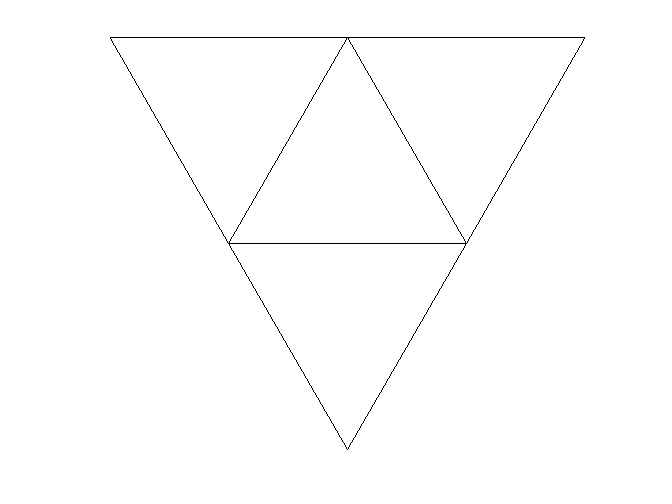
\includegraphics[scale = 0.5]{flattetrahedron.png}
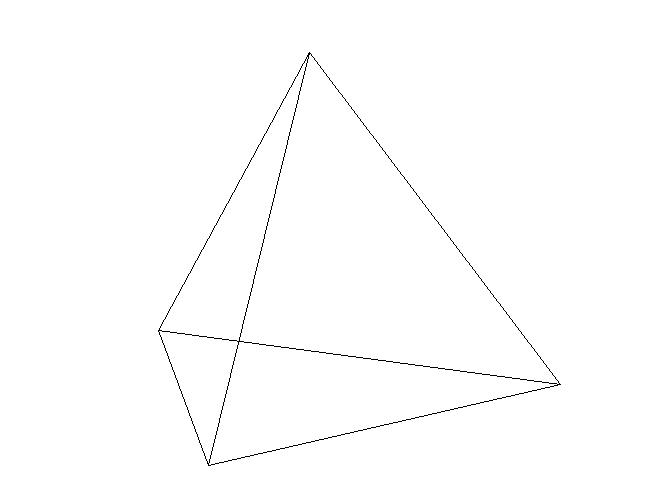
\includegraphics[scale = 0.3]{tetrahedron.jpg}
\caption{An example of a triangulation. The triangles can be folded up into the boundary of a tetrahedron.}
\end{figure}

\subsection{Definitions}
\maketitle

We begin by providing the definition of a manifold. A manifold is defined as any topological space containing points whose neighborhoods are topologically equivalent to the open unit ball, or as we say resemble Euclidean space. The idea of manifolds is broad enough to encompass many different types of spaces that may exist in \textit{n} dimensions. We may classify different types of manifolds by topological equivalence. One term we can use to generally describe manifolds is "locally Euclidean". With this in mind, one may be able to examine the properties of a manifold, what may be a potentially large and complex space, by examining its behavior locally.\newline

\noindent One way to do this is to represent our manifold that we are observing using a topological triangulation. On an $n$-dimensional manifold, this triangulation, written $\tau = {\tau_0, \tau_1, ... , \tau_n}$ consists of lists of simplices $\sigma^k$, where the super-script denotes the dimension of the simplex and $\tau_k$ is the list of all \textit{k}-dimensional simplices $\sigma^k = {i_0, ... , i_k}$ \cite{Dave}. We shall refer to 0-dimensional simplices as vertices, 1-dimensional simplices as edges, 2-dimensional simplices as triangles or faces, and 3-dimensional simplices as tetrahedra.\newline

\noindent For the purpose of this project, it will not be necessary to look at simplices of higher dimensions. However, concepts may translate to all dimensions. Primarily, we will be working exclusively with 2-dimensional manifolds, or surfaces, and eventually we will address these problems in 3-dimensional manifolds. Additionally, we are only concerned with manifolds that are closed, or without boundary. \newline

\noindent When talking about closed, triangulated surfaces an important characteristic comes up that is known as the Euler characteristic, given by the equation $\chi = V - E + F$, where \textit{V} is the number of vertices in the triangulation, \textit{E} is the number of edges, and \textit{F} is the number of faces. This characteristic is directly connected to another important property which is the \textit{genus} of a surface. The genus of a surface is a number that describes the toplogical property that is more loosely known as the number of ``holes'' in the surface. For instance, a sphere has a genus of 0 while a torus has a genus of 1, a two-holed torus has genus 2, etc. The relationship between the two values is given by $X = 2 - 2g$, where \textit{g} is the genus of the surface.\newline 

\begin{table}
\begin{tabular}{lccccc}
Name  &	Vertices, V &	Edges, E & Faces, F &	Genus, g & $\chi$\\
\hline 
Tetrahedron &	4 &	6 &	4 &	0 & 2\\
Octahedron 	&	6 &	12 &	8 & 0 &	 2\\
Icosahedron &	12 & 30 & 20 & 0	&	 2\\
Torus & 9 & 27 & 18 &	1 & 0\\
Two-holed torus & 10 & 36 & 24 &	2 & -2\\
\end{tabular}
\caption{Listings of vertices, edges, faces, and genus for some common shapes}
\label{EuChar}
\end{table}

\noindent Just as we can say that a whole triangulation is composed of 2-dimensional simplices, we must make a definition for each individual simplex. For our data structure, we decided on creating a list of references for each simplex to give it definition within the triangulation. These lists of references for each simplex are refences to other simplices in the triangulation with the property of being local. We define the term ``local'' slightly different for each simplex. To begin with, we say that an edge is defined by two vertices and a face is defined by three vertices and three edges. Then, we can say that a vertex is local to any edge that it is in the definition of and any face that it is in the definition of, as well as any vertex that it shares an edge in common with. An edge is local to any vertex that it is defined by and any face that it is in the definition of, as well as any edge that it shares a vertex in common with. A face is local to any vertex it is defined by, any edge that it is defined by, and any face that it shares an edge in common with. These are the definitions for locality of simplices that we decided upon, creating three different lists for each simplex. From these definitions, we can come to certain conclusions about the amount of local simplices a given simplex can have. A vertex must have at least three local vertices, at least three local edges, and at least three local faces. An edge must have exactly two local vertices and exactly two local faces. A face must have exactly three local vertices, exactly three local edges, and exactly threee local faces. Some of these definitions do not hold true for one special case known as the double triangle, which will be addressed later on in the paper, but in all other cases, these properties hold.

\subsection{Circle packing}
\maketitle

\noindent Given a triangulation, we wish to assign lengths to edges. This is known as adding a metric to the triangulation. One way to do this is to create a \textit{weighted triangulation}. This is done by a technique called circle-packing. Visually, circle-packing entails placing circles with their centers on a vertex so that neighboring circles are tangent to each other. That is, they intersect at only one point, as shown in Figure \ref{rightTri}. The radius of the circle at a vertex, $v_i$, is known as its weight, $r_i$. For any lone triangle, this can be done. By applying weights to each vertex we provide lengths to the edges of our triangulation as $l_{ij}=r_i+r_j$, where $r_i$ and $r_j$ are the radii of the circles centered at vertices $v_i$ and $v_j$, and $l_{ij}$ is the edge with vertices $v_i$ and $v_j$. The metric applied to the triangulation in this way, with Euclidean triangles (see $\oint\ref{HypSphere}$), is known as the \textit{cone metric} \cite{chowluo}.\newline

\noindent Choosing to define the metric in this way, we guarantee the triangle inequality and ensure that we are creating triangles. It is also needed to run the Ricci flow, explained in $\oint\ref{ricciDef}$. But, there are restrictions to applying weights first. Not all combinations of edge lengths are possible under this system. Some triangles can simply not be circle-packed. The most common example is shown in Figure \ref{rightTri}, where there is no combination of weights at the vertices that can make a proper circle-packing. By allowing generalizations of circle-packings, as discussed in $\oint\ref{circExt}$, we can broaden our range of possible length assignments.

  
\begin{figure}
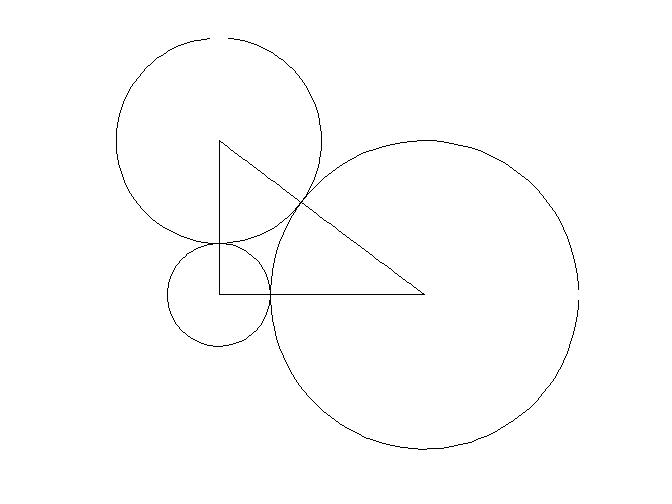
\includegraphics[scale = 0.3]{righttriangulation.jpg}
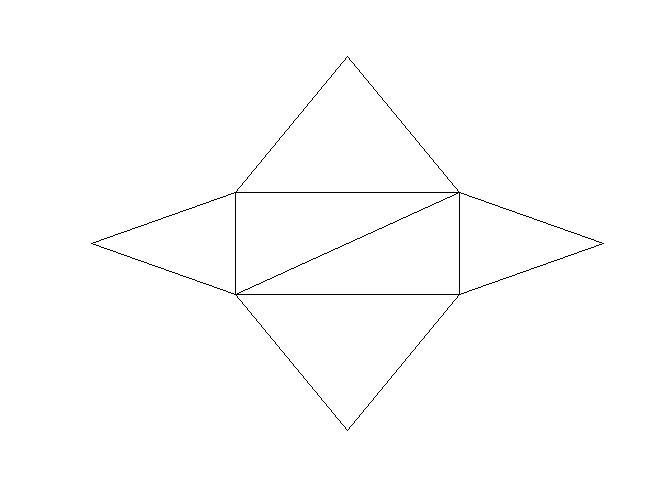
\includegraphics[scale = 0.3]{badcase.jpg}
\caption{An example of circle packing (left) and a triangulation that cannot be circle-packed.}
\label{rightTri}
\end{figure}

\subsection{Duals}
\maketitle

Every triangle has a circle that is internally tangent to all three edges. This $incircle$ is perpendicular to each circle centered at one of its vertices, and has a radius $\displaystyle r = \sqrt{\frac{(s-a)(s-b)(s-c)}{s}}$ where $s$ is the semi-perimeter of the triangle, and $a, b, $and $c$ are the side lengths. Let us rewrite this in terms of the vertex weights, since we are using circle packing. Thus, a side length is simply the sum of two vertex radii. We can then simplify this equation to $\displaystyle r = \sqrt{\frac{r_i r_j r_k}{r_i + r_j + r_k}}$, with $i, j$ and $k$ being the vertices of the triangle. This can be done on each triangle. All these incircles are mutually tangent to each other, and any line connecting two adjacent incircles is perpendicular to the common edge of the two triangles. We define the length of this dual edge $\star e$ as the sum of the radii of adjacent incircles. $\star e = r_{in1} + r_{in2}$. Every edge has a dual length. See Figure~\ref{fig:dual} for an illustration of a dual edge.\newline

\noindent With the dual edges, we can obtain a polygon surrounding each vertex. The area of the region formed by these duals is called the dual area, calculated by $$\star A_i = r_i\sum{\frac{\star e_i}{2}} = r_i\sum{r_{\mbox{inscribed}}}$$ where $r_i$ is the weight of the vertex. The sum is over all faces incident to vertex $i$.\newline

\noindent The dual length and dual area have some interesting properties that we hope to investigate. David Glickenstein examines these and more in \cite{Dave}. 

\begin{figure}
\centering
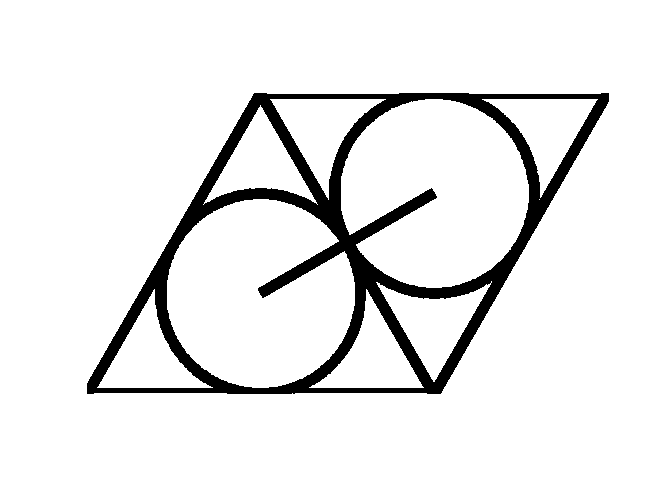
\includegraphics[scale = 0.4]{dual.png}
\caption{A dual to an edge}
\label{fig:dual}
\end{figure} 

\section{Ricci flow}
\subsection{Background}
Introduced by Richard Hamilton in 1982, Ricci flow, named in honor of Gregorio Ricci-Curbastro \cite{RicciBkgd}, has since had a large influence in the world of geometry and topology. It is often described as a heat equation. Imagine a room where a fireplace sits in one corner and a window is open on the other side. The heat will diffuse through the room until the temperature is the same everywhere. With Ricci flow, the same occurs with the curvature. Under Ricci flow, a geometric object that is distorted and uneven will morph and change as necessary so that all curvatures are even.The biggest consequence of Ricci flow came when Grigori Perelman proved the Poincar\'{e} Conjecture in 2002. The Poincar\'{e} Conjecture, proposed in 1904, was particularly difficult to prove, and was given the honor of one of seven millennium puzzles by the Clay Mathematics Institute. It was Ricci flow that turned out to be the cornerstone for the proof. In addition, its relation to the heat equation may open new doors for work in fluid dynamics and even in the theory of general relativity \cite{RicciBkgd}. In 2002, Chow and Luo introduced the concept of combinatorial Ricci flow. They showed that this new concept, performed on a triangulation of a manifold, had many of the properties of the Ricci flow Hamilton had defined. That the subject is still very new makes this research project exciting.

\subsection{Definition}
\label{ricciDef}

Just because we have a triangulation and that it is circle packed does not mean that it is in a desired configuration. Vertices can be too large or too small, and the resulting geometry can be somewhat intractable. We would like to have a way to determine the evolution of each shape to its final form, which may be more uniform. In their paper, Chow and Luo introduce an equation known as combinatorial Ricci flow. On a discrete surface, this equation allows the weights to change over time \cite{chowluo}. We introduce this equation to the reader which can be written as

  \begin{equation}
  \label{Riccif}
  \frac{dr_i}{{dt}} = -K_ir_i
  \end{equation}
  
\noindent where $K_i$ is a characteristic called the $curvature$ of a vertex, and $r_i$ is the $radius$ or $weight$ of the vertex $i$. We use the words ``radius'' and ``weight'' interchangeably, denoting the length of the radius that surrounds a vertex $i$ in circle-packing. The value of $K_i$ changes with time. Its value is found by determining the angles of all triangles containing vertex $i$. Using side lengths we can determine the angle using the law of cosines. For a triangle with lengths $a, b,\mbox{ and }c,$ the angle opposite side $c$ is
  
  $$
  \angle C = \arccos(\frac{a^2 + b^2 - c^2}{2ab})
  $$
  
\noindent with similar formulas for the other angles. We take the sum of all angles associated with a vertex $i$ and define the curvature $K_i$ as

\begin{equation}
K_i = 2\pi - \sum{\angle i}.
\end{equation}
  
\noindent Since we are performing multiple non-linear differential equations as variables depend on the weights which change over time, we can probably not solve them explicitly.\newline
   
\noindent A potential issue we noted is that, based on the equation, is it possible that the radii could continually decrease. Take, for example, a simple tetrahedron with all sides of equal length. We find that the curvature of each vertex always equals $\pi$. Thus in solving the differential equation computationally we would decrease each vertex by the same amount, but the curvature of each vertex would still remain $\pi$ because the curvature is not affected by uniform scaling. The radii would continue to decrease until they approach zero length. We have to address that issue since computers don't like working with numbers near zero, as in the denominator of the arccosine function. Numerical instability may occur. To avoid this issue, let us resize the length of each radius by a scalar, $\alpha$. We denote each scaled length by $\tilde{r_i}$ and equate as
 
 \begin{equation}
 \tilde{r_i} = \alpha r_i.
 \end{equation} 
 
\noindent Each $\tilde{r_i}$ would have its own $\tilde{K_i}$, but since we are scaling all sides by the same factor, this does not effect the curvature of the surface, so $\tilde{K_i} = K_i$. Thus in plugging $\tilde{r_i}$ in to the differential equation we get
 
 \begin{eqnarray}
 \label{ref1}
 \frac{d\tilde{r_i}}{dt} &=& \frac{d(\alpha r_i)}{dt} = \alpha \frac{dr_i}{dt} + r_i\frac{d\alpha}{dt}\nonumber\\
 &=& -\alpha K_ir_i + \frac{\tilde{r_i}}{\alpha}\frac{d\alpha}{dt} \nonumber \\
 &=& -\tilde{K_i}\tilde{r_i} + \frac{\tilde{r_i}}{\alpha}\frac{d\alpha}{dt}.
 \end{eqnarray}
 
\noindent We also note that $\displaystyle \frac{1}{\alpha} \frac{d\alpha}{dt} = \frac{d(\log \alpha)}{dt}$ using a basic chain rule. In order to find an appropriate value for $\alpha$ we decided to use the following criterium:
 
\begin{equation}
\label{eqprod}
f(\tilde{r_1},\tilde{r_2},\ldots,\tilde{r_n}) = \prod{\tilde{r_i}} = \prod{\alpha r_i} = C\mbox{, a constant.}
\end{equation}

\noindent We will call this value the \textit{product area} of the surface. This area prevents all radii from decreasing to zero at the same time. By taking the derivative of Eq.~($\ref{eqprod}$) with respect to time we find that 
 
\begin{equation}
\label{proof1}
\frac{d(\mbox{log}~\alpha)}{dt} = \frac{\mbox{sum of all curvatures}}{\mbox{number of vertices}} = \overline{K}, \mbox{average curvature.}
\end{equation}

\noindent In this paper, we may refer to the sum of all curvatures as the \textit{total curvature}. We can also show that $\overline{K}$ is a constant and depends on the number of vertices and the Euler characteristic. We know that the sum of angles from each vertex is 360 $\deg,$ or $2\pi$. However, we also know that the sum of angles on each face is $\pi$, thus we determine that 

$$\sum{K_i} = 2\pi V - \pi F = 2\pi(V - \frac{F}{2})$$

\noindent We can simplify this by noting trends in basic triangulations. As every face is made up of three edges, and each edge belongs to two faces, we can see that $3F = 2E, \mbox{or } E = \frac{3F}{2}$. Looking back at Table \ref{EuChar} we note this true for all polyhedra listed. Let us use this substitution and rewrite the above equation as

$$\sum{K_i} = 2\pi(V - \frac{F}{2}) = 2\pi(V - \frac{3F}{2} + F) = 2\pi(V - E + F) = 2\pi \chi.$$

\noindent Thus we find that $\overline{K}$ is just $\displaystyle\frac{\sum{K_i}}{|V|} = \frac{2\pi \chi}{|V|}$ where $|V|$ is the number of vertices. This is also noted in \cite{chowluo}. Plugging this information back into Eq.~($\ref{ref1}$) we determine that

\begin{equation}
\frac{d\tilde{r_i}}{dt} = -\tilde{K_i}\tilde{r_i} + \overline{K}\tilde{r_i} = (\overline{K} - \tilde{K_i})\tilde{r_i}
\end{equation}

\noindent However, since everything is now a function of $\tilde{r_i}$ and not $\alpha$, we can just as easily plug $r_i$ back in to the differential equation instead of $\tilde{r_i}$, so we end up with:

\begin{equation}
\label{Riccin}
\frac{dr_i}{dt} = (\overline{K} - K_i)r_i
\end{equation}

\noindent This is known as normalized Ricci flow, as discussed in \cite{chowluo}. In the case of our basic tetrahedron from earlier, the radii would not change after each iteration as $\overline{K} = K_i = \pi$ and thus $\displaystyle\frac{dr_i}{dt} = 0$ for $i = \{1,2,3,4\}$. 

\subsection{Expectations}

We have some expectations for combinatorial Ricci flow over two-dimensional Euclidean surfaces. Cases like the boundary of the tetrahedron can be calculated by hand so it will be useful to test our results against these surfaces. For example, we expect that the tetrahedron under (\ref{Riccif}) will have all weights converge to zero. Whereas under (\ref{Riccin}) the weights are expected to converge to positive constants.\newline

\noindent There are other expected behaviors. We expect that the product of the initial weights will be equal to the product of the weights at any intermediate step of the flow, what we call the \textit{product area}. Also, it is predicted that the total curvature of a 2-manifold surface should remain a constant determined by its genus.\newline

\noindent For the program we expect to create a system that allows for easy access of information while also providing that information in a time efficient way. Our goal is to create a program that can be built upon later to provide further functionality and options without requiring widespread and time consuming changes to the code. While we certainly expect a number of bugs, we plan to develop methods to test and find any errors in our code. \newline


\noindent Initial checks for accuracy:
\begin{enumerate}
\item Boundary of tetrahedron will converge to equal weights.
\item Constant \textit{product area}.
\item Constant total curvature.
\end{enumerate}

\section{Program/Code}
\label{Programchap}
\subsection{Structure}


When creating the program, the data structure design was critical. The design not only helps dictate the direction of the project over the course of its lifespan, but the decisions affect the speed and efficiency of all added functionality. It was agreed that the system would have to hold the different simplices and that they would be referencing each other. This part of the program would need to be structured in a way that makes it quick and easy to move from one simplex to another. As seen in Figure \ref{triUML}, all simplices are assumed to have lists of references to other simplices, what we call local simplices, broken down by dimension. For the two-dimensional case, each simplex has lists of local vertices, local edges, and local faces..\newline
  
\begin{figure}[ht]
\begin{center}
\includegraphics[scale = 0.50]{triangulationUML.png}
\end{center}
\caption{A UML diagram of the program. The UML shows how the various files interact as well as the functions and variables they hold.}
\label{triUML}
\end{figure}

\noindent The lists are vectors of integers. The vector, provided in the C++ library, was chosen so that the list can dynamically change in size. The integers are a decision based on both speed and size. Instead of, for example, a vertex having a list of actual edges ($\overline{AB}, \overline{CF},$ etc.) or pointers to edges, the vertex has a list of integers representing the edges. The actual edges are then obtained through the $Triangulation$ class, which holds maps from integers to simplices. The $Triangulation$ class is made up of static functions and maps and is designed so only one triangulation exists at any time. Because the maps are static, they can be accessed at any time from anywhere in the code without the need to pass pointers through function calls. Vertices also hold a weight, representing the radius from a circle packing on the triangulation. Edges then have a length based on the weights of its two vertices. When a vertex's weight is changed, the local edges to that vertex update their lengths automatically.\newline


\noindent While we are able to manually construct a few basic triangulations by hand, as we add more vertices doing so will become harder. Frank Lutz, creator of The Manifold Page \cite{lutzmanifold}, has a little under two million known triangulations of varying sizes. However, the format is different than our setup, so we developed an algorithm to take a given triangulation, saved on its own as a text file, and convert it into the form that we use. We were able to transform this
  
\begin{verbatim}{manifold_lex_d2_n5_o1_g0_#1=[[1,2,3],[1,2,4],[1,3,4],
[2,3,5],[2,4,5],[3,4,5]]}
\end{verbatim}
 
\noindent which solely documents the faces, into our format, which can be seen in Table~\ref{tab:format}.

\begin{table}
\begin{center}
\begin{tabular}{|l|l|l|}
\hline
 Vertex: 1 &    Edge: 1 &    Face: 1 \\ \hline 

     2 3 4 &        1 2 &     1 2 3  \\

    1 2 4  & 2 3 4 5 7  &     1 2 3  \\

    1 2 3  &       1 2  &     2 3 4  \\ \hline 

 Vertex: 2 &    Edge: 2 &    Face: 2 \\ \hline

   1 3 4 5 &        1 3 &     1 2 4  \\

  1 3 5 7  & 1 3 4 6 8  &     1 4 5  \\

  1 2 4 5  &       1 3  &     1 3 5  \\ \hline 

 			\vdots & \vdots & \vdots \\ \hline 

 Vertex: 5 &    Edge: 9 &    Face: 6 \\ \hline

     2 3 4 &        4 5 &     3 4 5  \\

    7 8 9  & 4 5 6 7 8  &     6 8 9  \\

     4 5 6 &       5 6  &     3 4 5  \\
\hline
\end{tabular}
\end{center}
\caption{Conversion of format from \cite{lutzmanifold} to ours.}
\label{tab:format}
\end{table}  

\subsection{calcFlow}

\noindent The function $calcFlow$ runs a combinatorial Ricci flow on a triangulation and records the data in a file. The algorithm for solving the ODE, provided by J-P Moreau, employs a Runge-Kutta method of order 4 \cite{JPM}. First, the file name for the data is provided. Then, a $dt$ is given by the user that represents the time step for the system. The next parameter is a pointer to an array of initial weights to use. This is followed by the number of steps to calculate and record. Lastly, a boolean is provided, where $true$ indicates that the normalized differential equation, (\ref{Riccin}), should be used. Otherwise, the standard equation (\ref{Riccif}) is employed. Each step, with every vertex's weight and curvature at that step, is printed to the file. An example is shown in Table~\ref{tab:ricciSteps}.\newline

\begin{table}
\begin{center}
\begin{minipage}{2.2in}
%\begin{multicols}{2}
\begin{tabular}{l|l|l}
\hline
Step 1   & Weight &  Curv\\
Vertex 1:& 6.000 & 0.7442\\
Vertex 2: &3.000 & -1.122\\
Vertex 3:& 3.000 & -1.373\\
Vertex 4:& 8.000 & 1.813\\
Vertex 5: &6.000 & 1.227\\
Vertex 6: &2.000 & -3.046\\
Vertex 7: &4.000 & -0.3045\\
Vertex 8: &8.000 & 1.989\\
Vertex 9: &5.000 & 0.07239\\ \hline
\end{tabular} 
\end{minipage}
\begin{minipage}{2.2in}
\begin{tabular}{l|l|l}
\hline
Step 50 &  Weight &  Curv\\
Vertex 1:& 4.557 & 0.008509\\
Vertex 2: &4.530 & -0.01185\\
Vertex 3: &4.534 & -0.009091\\
Vertex 4:& 4.563 & 0.01268\\
Vertex 5:& 4.550 & 0.002772\\
Vertex 6: &4.527 & -0.01455\\
Vertex 7: &4.541 & -0.003563\\
Vertex 8: &4.559 & 0.01018\\
Vertex 9: &4.553 & 0.004906\\ \hline
\end{tabular}
\end{minipage}
%\end{multicols}
\end{center}
\caption{Two steps of a Ricci flow}
\label{tab:ricciSteps}
\end{table}

\noindent After the initial design of $calcFlow$, tests were run to determine its speed. The time it took to run was directly proportional to the number of steps in the flow. However, it was also proportional to more than the square of the number of vertices of the triangulation. As a result, while a four-vertex triangulation can run a 1000 step flow in three seconds, it would take a twelve-vertex triangulation 43 seconds to run the same flow. After inspecting the speed of the non-adjusted flow in comparison, it became clear that the calculation of total curvature, which remains constant in two-dimensional manifold cases, was being calculated far too often. After being adjusted so that it is calculated just once per step, the speed of the flow is much faster so that a four-vertex system with 1000 steps takes just one second and twelve vertices is much improved with a time of only four seconds. The code for the $calcFlow$ function can be found in $\oint\ref{calcFlowCode}$.

\subsection{Morphs}

Another part of the code is a file strictly made up of functions used to manipulate and alter the triangulations being run. These functions, known within the code as \textit{morphs}, allow us to change the triangulation in different ways, geometric as well as topological, in order to provide us with different kinds of discrete manifolds over which to run our flow.

\subsubsection{Flips}

One type of morph that we have available is known as a flip, called this because the transformation appears equivalent to the change in the planar projection of a tetrahedron when it is flipped over completely. Known also as \textit{bistellar moves}, these transformations can be used to change the degree of a particular vertex or many vertices, or coarsen or refine an entire triangulation as a whole. In higher dimensions, there are many different moves of this kind, but in two dimensions, we have only three types.

\begin{itemize}
\item 1-3 flip \newline
In a 1-3 flip, a single face is replaced by three faces. One way to think of going about this procedure is to simply add a new vertex to an existing face. This requires creating three new edges that connect the new vertex to the three vertices of the existing face.
\item 2-2 flip \newline
In this flip, we take a pair of adjacent faces and readjust the edge that they share to connect the opposite pair of vertices, as shown in figure~\ref{fig:flip}. This move creates no new simplices and removes no existing vertices. The code for the 2-2 flip is located in $\oint\ref{calcFlowCode}$.


\begin{figure}
\centering
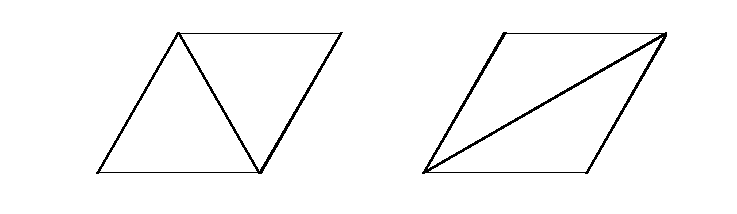
\includegraphics[scale = 0.8]{Flip.png}
\caption{An example of a 2-2 flip.}
\label{fig:flip}
\end{figure}

\item 3-1 flip \newline
In what is essentially the inverse of the 1-3 flip, the 3-1 flip is one where we take a vertex that is connected to three other vertices and remove it entirely. This move is more restrictive than the others since not every vertex is connected to exactly three vertices. 
\end{itemize}
Flips have the special property that they do not change the Euler characteristic of the surface they are performed upon. For example, in performing a 1-3 flip, we have a total of 3 new edges, 2 more faces, and 1 new vertex. The value of $\chi$ does not change as $(V+1) - (E+3) + (F+2) = V - E + F = \chi$. This means we could do any number of these flips without changing the topology of the surface. \newline

\noindent Another thing of note is that any flip we could think of (2-5 flip, 1-4 flip) could be made using a combination of 1-3, 2-2, and 3-1 flips. Thus these three seem to generate all possible configurations.
  

\subsubsection{Other Transfigurations}

In addition to the flips that were described above, there are other ``morphs'' that can be performed to change the topology of a triangulation in order to give us some more diverse and interesting shapes over which to run these flows and observe their results. There are two such moves that we can perform.

\begin{itemize}
\item Adding Handles \newline
By adding a handle to a surface, we are in essence adding a hole to it. One simple way to obtain this result is to ``patch'' the surface of a torus to the surface that we are working with. This is exactly what we have done. The method removes a face from the existing triangulation and replaces it with a 9-vertex triangulation of a torus. By using the three existing vertices and edges, we are actually adding 6 new vertices, 24 new edges, and 17 new faces. This operation changes the topology of the triangulation that we are working with. It will reduce the Euler characteristic, $\chi$, by 2 and thus change the total curvature of the figure.
\item Adding Cross-Caps \newline
A cross-cap is a piece of a surface with a self intersection. The purpose of adding a cross-cap to a manifold is to give us a property of non-orientability. A surface of this kind is characterized by the ability to move an object along it in such a way that it reaches its original location but in mirror-image form. In this way, the portion of the surface known as the cross-cap is, itself, topologically equivalent to the mobius band. It is sufficient to add only a single cross-cap to any given surface,. In conjunction with the method of adding handles, this technique allows us to create any topology in two dimensions.
\item Adding Double Triangles \newline
Another shape we have been looking into is called the double triangle. A double triangle is made of two triangles with the same three vertices. It can also be thought of as folding one triangle on top of another. We can add these to a triangulation and see how things vary with their presence. This is of interest because of their very peculiar effect on the definition of a triangulation. Without double triangles, there are certain restrictions on definitions and adjacency properties of simplices within a triangulation as outlined in the previous section on triangulations. However, with these double triangles, the restrictions are broken up by allowing double and even triple adjacency references, creating vertices with only one or two local vertices, faces with only two defining edges, and edges with only one defining vertex, among other bizarre properties. Because of these inconsistencies in definition, different surfaces that have these double triangles attached to them will behave in noteworthy ways. The function that adds these shapes takes an edge as an argument and adds another edge with the same two vertices. Then, a vertex is added and two edges are drawn from this vertex to the other two vertices mentioned. Two new faces are formed by these two new edges as well as the other two edges mentioned, one for each face. The process can be imagined as flattening a party hat and attaching it to an object along the open end.
\end{itemize}

\section{Results}

\subsection{Flows}

The program for the Ricci flow was tested by beginning with the simplest cases, and then explored with as many different possibilities as we could conceive of to try to find anomalies. The first test was the boundary of the tetrahedron. In the standard equation, it is easily shown that all weights approach zero exponentially fast. In the normalized equation, and the equation that is used in the rest of the testing, the tetrahedron's weights approach a single positive number, the fourth root of the \textit{product area} of the tetrahedron, so that the area remains constant. In addition, all the curvatures converged to the same value, in this case $\pi$, so that the total curvature is $4\pi$. Results were similar for the other platonic solids.\newline

\noindent The next test was the torus with the standard nine-vertex triangulation. Again all the weights approached the same positive number to maintain constant area. As expected, the curvatures all went to zero while the total curvature remained zero throughout. Further simple tests included triangulations of larger genus, and in all cases the total curvature remained at a constant multiple of $\pi$ that was expected and the \textit{product area} was also constant. In addition, there does not appear to be any further effect from the initial weights other than determining the area of the triangulation. It is not clear from any of the tests we ran that having extremes amongst the initial weights causes a different end result.\newline

\noindent In each case all vertices converged to the same curvature. This was not always the situation for the weights, as in many triangulations there would be several final weights. It became clear that this would occur when vertices had different degrees. In fact, we guess that there is a formula relating the \textit{product area} of a weighted triangulation and the degree of a vertex to that vertex's final weight. In most of the examples we tried, when two vertices had the same degree, they had the same final weight, but this is not always the case. One such example is adding three vertices to one face of the tetrahedron. As seen in Table \ref{tab:weightTab}, vertices 4, 5, and 6 all have degree four. Yet vertex 5 has a greater final weight than the other two. The only explanation we could find with some merit is that the local vertices of 5 are different in degree from those of 4 and 6. That is, the degrees of the local vertices of 5 are never less than four, while vertices 4 and 6 each have a local vertex with degree 3. See Figure \ref{fig:t7vh} in the Appendix for an illustration of weights over time.\newline 


\begin{table}

\begin{minipage}[ht]{0.5\linewidth}

\begin{tabular}{|l|l|}
\hline
 Vertex: 1 &  Vertex: 5 \\
\hline
2 3 4 5 6 7  &   1 2 4 6  \\

1 2 3 7 10 13  &  7 8 9 12  \\

1 2 3 5 7 9  &   5 6 7 8  \\
\hline
 Vertex: 2 &  Vertex: 6 \\
\hline
1 3 4 5 6 7  &   1 2 5 7  \\

1 4 5 8 11 14  & 10 11 12 15  \\

1 2 4 6 8 10  &  7 8 9 10  \\
\hline
 Vertex: 3 &  Vertex: 7 \\
\hline
    1 2 4  &     1 2 6  \\

    2 5 6  &  13 14 15  \\

    2 3 4  &    1 9 10  \\
\hline
 Vertex: 4 &  Edge: 1    \\ 
\hline
  1 2 3 5  &   :         \\

  3 4 6 9  &   :         \\

  3 4 5 6  &            \\ 
\hline

\end{tabular}


\end{minipage}
\begin{minipage}[b]{0.5\linewidth}

\begin{tabular}{|l|}
\hline
Final weights for a random \\

initial weighted Triangulation \\
\hline
Vertex 1: 15.692 \\

Vertex 2: 15.692 \\

Vertex 3: 6.18421 \\

Vertex 4: 9.6524 \\

Vertex 5: 10.6409 \\

Vertex 6: 9.6524 \\

Vertex 7: 6.18421 \\
\hline
\end{tabular}
\end{minipage}
\caption{Adding three vertices to a Tetrahedron}
\label{tab:weightTab}
\end{table}


\subsection{Specific cases}

\noindent Example: Adding a vertex to a one-holed torus. See figure~\ref{torusaddv}. \newline

\noindent By inserting a vertex within a triangulation for a torus, we are essentially creating a bump on the torus and then observing what happens as we run it through out $calcFlow$ program. We discovered that the new vertex shrinks in size to a weight much smaller than the other vertices, but to a positive constant. To counter this, the other vertices grow slightly to maintain Eq.~(\ref{eqprod}). The weight that the new vertex converges to turned out to be in proportion to the other weights by $3+2\sqrt{3}$, the exact proportion necessary to maintain equality amongst all other weights. An oddity here is that the three vertices local to this added vertex converged to the same weight as all the vertices not near the flip, despite a difference in degree.\newline

\begin{figure}[ht]
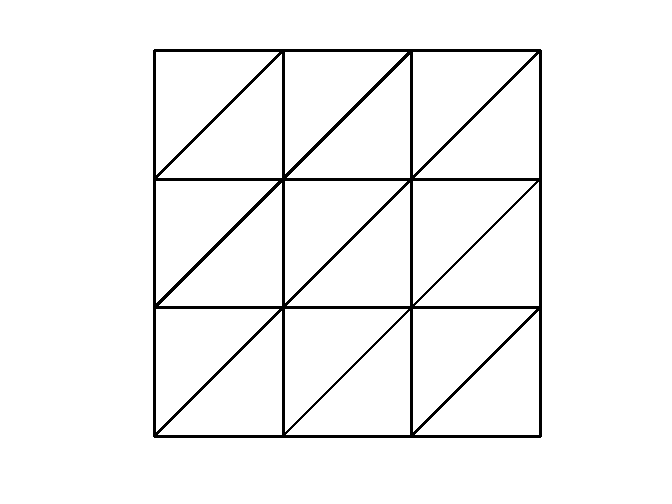
\includegraphics[scale = 0.5]{torus22.png}
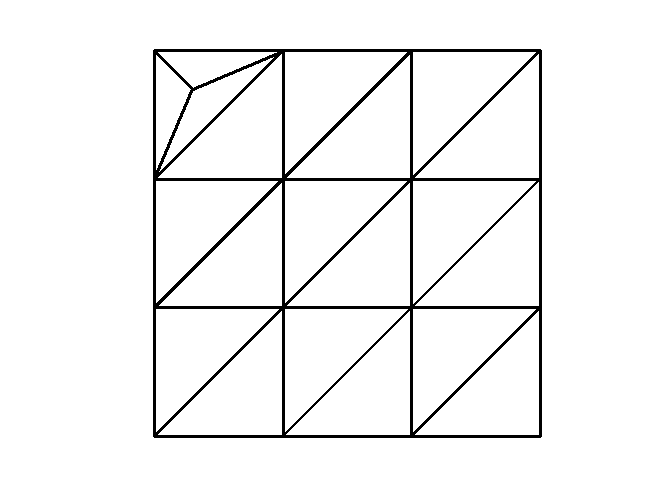
\includegraphics[scale = 0.5]{torus2addvertex2.png}
\caption{A triangulation of the torus, and the addition of a new vertex. This is a 1-3 flip.}
\label{torusaddv}
\end{figure}

\noindent Example: Adding a leaf to a two-holed torus.\newline

\noindent When we added a double triangle to the edge of a two-holed torus, we experienced for the first time what is known as a singularity. At the special vertex that was only of degree two, its weight continued to shrink and never converged. Eventually, enough steps of the Ricci flow were performed that the size of the weight became less than what the computer could differentiate from 0 and the program crashed with a division-by-zero error. Before the crash, the other vertices were increasing without convergence to counteract the decreasing weight. The reason is that all vertices wanted to attain the same curvature, in this case $-\frac{2}{5}\pi$. Yet the new vertex, with only two angles in its sum, can only obtain a curvature of 0 (each angle $\sim\pi$ radians). The result is that the weight shrinks in an attempt to attain angles greater than $\pi$, which is simply not possible. What is still not clear is whether or not the weight reaches 0 in finite time, or simply approaches 0. This is difficult to test with a computer only capable of approximating the weight, though we expect that it does so in finite time.\newline

\noindent Example: Performing a 2-2 flip on a 12-vertex torus. \newline

\noindent One interesting observation we made was that flips can drastically change the behavior of some triangulations. For Example, in a 12-vertex torus, performing a flip on one edge affected created a double triangle. Similarly to the previous case, all curvatures are converging to 0, but the vertex with degree 2 simply cannot accomplish this. However, unlike the previous case, we suspect that the weight does not become 0 in finite time, but instead approaches 0.\newline

\noindent Example: Triangulation of genus 4.\newline

\noindent While the previous two cases were quite interesting, there is some hesitation given that we were using double triangles and being less restrictive in what were allowable triangulations. But the theory behind why both situations reacted as they did left hope for a case that fit in a stricter setting. In the same sense that a two degree vertex could have a curvature no less than 0, a three degree vertex is bounded below by $-\pi$. It was observed that the vertices of a triangulation all converge to $\displaystyle\frac{2\pi\chi}{|V|}$ curvature. Now it was a matter of finding a triangulation with a large enough genus and few vertices. The first we found, provided by \cite{lutzmanifold}, was an 11 vertex triangulation with genus 4. To create a vertex with degree 3, we chose to add a new vertex to a face with a 1-3 flip. This made all curvatures try to converge to $-\pi$. We then expected that the new vertex would react as in the previous example. This was in fact the case, and it presents the question of whether or not there is a limit on the degree that can create such a singularity. The issue being that for higher genus, more vertices are required. Unfortunately, \cite{lutzmanifold} does not provide large enough triangulations for fourth degree vertices. A data plot of this situation with a genus 6 triangulation is provided in $\oint\ref{dataplots}$. \newline

\noindent Example: Two tetrahedra connected at a vertex. See Figure \ref{fig:tt}\newline

\noindent It turns out $\chi = $7 Vertices - 12 Edges + 8 Faces = 3, which is not a case we had seen before. In previous cases $\chi$ was an even integer. Starting each vertex with equal weight, we obtained an unexpected result. The center weight becomes very large, and the others become smaller in comparison. We concluded that since the central vertex has a much higher degree, its weight becomes large, creating elongated tetrahedra on either side, in order to have the same curvature as all other vertices. One good thing we noted was that the net curvature = $6\pi = 2\pi\chi$.  

\begin{figure}
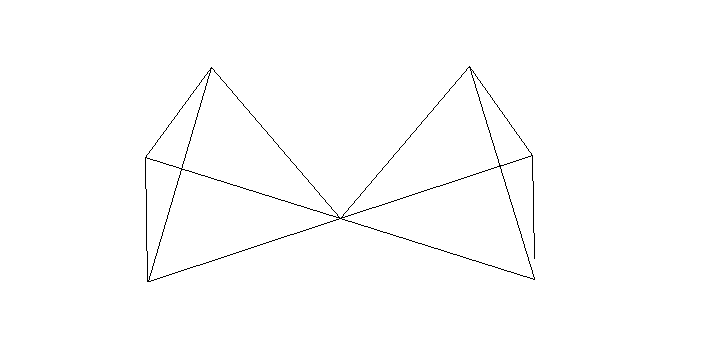
\includegraphics{tetratouch.png}
\caption{Two tetrahedra conjoined at a vertex.}
\label{fig:tt}
\end{figure}

\subsection{Convergence speeds}

One experiment we performed was measuring convergence speeds of various triangulations. For each triangulation, five flows were run where the weights were random between one and twenty-five. Random weights, while not a perfect solution, was the most effective option and easiest to implement. It was unclear what set weights could have an equal effect for different triangulations. By performing five trials and using random weights, we hope to negate any effect the weights could have on the convergence speed of a triangulation. The $dt$ was held constant at 0.03 so that the number of steps needed to run was not large and time consumming and still provided accurate results. For each run, a step number was assigned for when all weights and curvatures had converged to four digits, (the precision shown in a file of the results).\newline

\begin{figure}
\centering
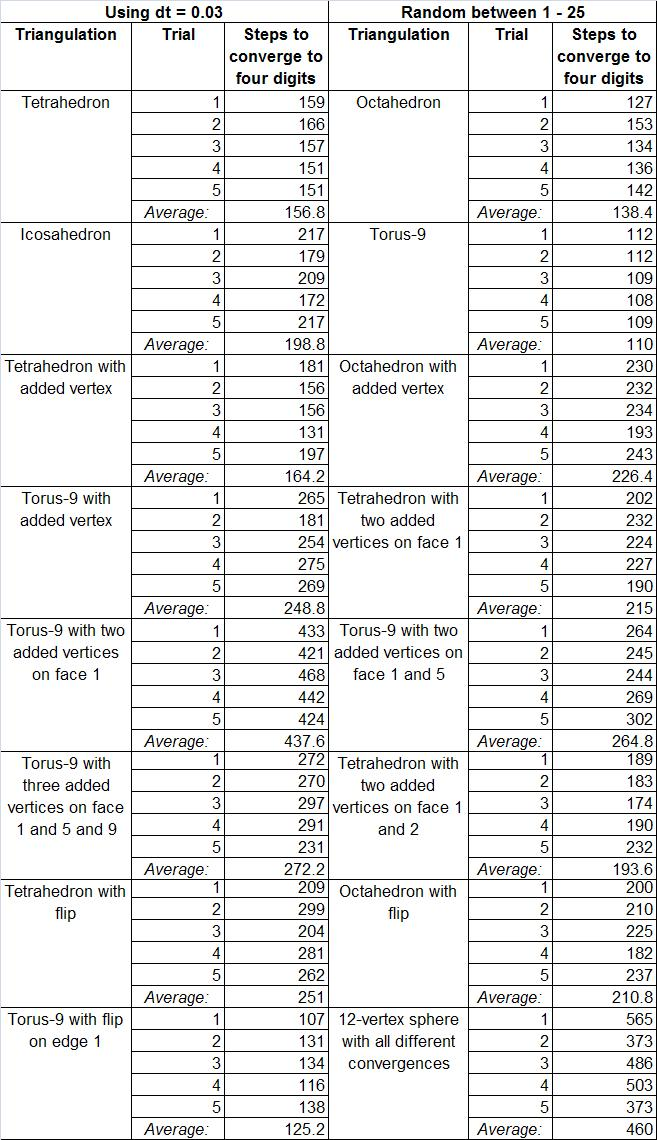
\includegraphics[scale = 0.79]{ConvergenceTable.png}
\caption{Summary of convergence data for varying criteria}
\label{fig:conv}
\end{figure}

\noindent Beginning with the basic case, the tetrahedron took on average 156.8 steps to converge to four digits and remained fairly consistent through all five trials. Strangely, the octahedron converged faster on all five flows, averaging 138.4 steps. This was made all the stranger by the fact that the icosahedron averaged 198.8 steps. The torus revealed several things about convergences. First, the standard nine vertex torus averaged only 110 steps, suggesting that a torus converges faster than a sphere. When a vertex was added to the torus, it greatly decreased the convergence speed, to 248.8 steps. Compared to the Tetrahedron with an added vertex, 164.2, this was a very large jump. When another vertex was added to the same face as the first, the convergence speed dropped yet again, to an average of 437.6 steps. Yet when this vertex was added to a face not connected to the first, the convergence speed was almost steady at 264.8. And adding a third in the same style caused little increase.\newline

\noindent This seems to suggest that convergence speed is dependent on the number of unique vertices. By unique we mean the properties of the vertex (number of local vertices, the weight it converges to, etc.). When the vertices were added to separate faces, there remained only three unique vertices. Whereas, adding the two vertices to the same face created five unique vertices. This theory is further supported by a twelve vertex sphere designed so that all vertices are unique. The average convergence was 460 steps, more than twice as long as the icosahedron, which also is a twelve vertex sphere.\newline

\noindent As a final note, the deviation of the initial weights did not have a clear impact on the convergence speed. At some times, it would appear that initial weights with a higher deviation would converge faster, yet at other times it was lower deviation that seemed to lead to faster convergence.

\section{Future work}
\subsection{3-D}

We would also like to start investigating 3-dimensional constructs built from tetrahedrons. We can adjust our current code as much as we need to, and ultimately be able to evaluate Yamabe flow, as discussed by \cite{DrG}. While Yamabe flow is similar to Ricci flow, its value of $K_i$ is determined quite differently, involving not only the angles of the faces, but also the cone angles associated with tetrahedron vertices.\newline

\noindent Ultimately, Dr. Glickenstein would like to be able to build 3-D representations of these surfaces and walk along them in any given path. We can look into how faces are connected to each other, and like a tesselation, be able to move from one triangle to another seamlessly. We can lay groundwork for that, and when this project is able to jump to 3-D modeling, we hope that this will help.  

\subsection{Circle packing expansions}
\label{circExt}
Circle packing is a very special way to characterize our side lengths. If we relax this criteria and let the circles overlap, we can introduce a second weight $\Phi$ that is representative of their angle of intersection. See Figure \ref{fig:intcirc}. We can then evaluate our side lengths as $$l_{ij} = \sqrt{r_i^2 + r_j^2 + 2r_ir_j\cos(\Phi(e_{ij}))}$$ With this more general interpretation, we can examine questions asked by Chow and Luo in \cite{chowluo}.  
%
\begin{figure}
\begin{center}
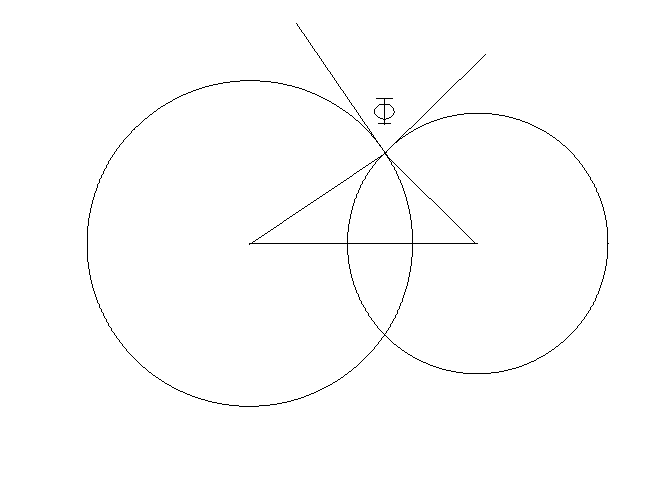
\includegraphics[scale = 0.6]{intcirc.png}
\end{center}
\caption{An example of relaxing circle packing and introducing $\Phi.$}
\label{fig:intcirc}
\end{figure}

%\begin{figure}
%\begin{center}
%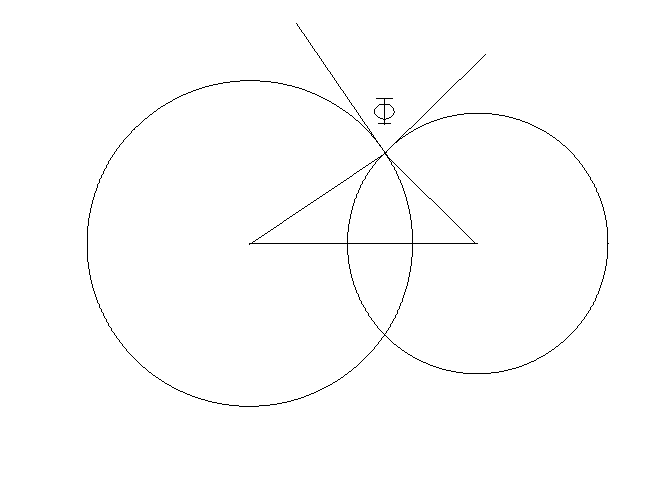
\epsfig{file=intcirc.eps,width=0.9\linewidth,clip=}
%\caption{An example of relaxing circle packing and introducing $\Phi.$}
%\label{fig:intcirc}
%\end{center}
%\end{figure}

\subsection{Hyperbolic/ spherical triangulations}
\label{HypSphere}
Hence far, we have focused on Euclidean triangles. However, there are cases when triangulations may be better suited in other systems. In changing our format to hyperbolic and spherical coordinates, we would have to reevaluate each of our steps depending on the system. For example, in hyperbolic, the basic Ricci flow equation is $\displaystyle \frac{dr_i}{dt} = -K_i\sinh r_i$. Note that in, for instance, spherical geometry, for a surface $X, \displaystyle \sum{K_i} = 2\pi\chi - \mbox{Surface Area of } X$, which can change over time. \newline

\noindent It is also of interest to run variations of our $calcFlow$ program based on our different geometries. We can observe whether or not each triangulation converges in the same fashion, or if it matters which geometry we choose. If we do discover that all systems behave the same way, we would then like to focus on one geometry, most likely Euclidean, as that would be easier to grasp and be more computational. 

\section{Conclusion}

We had a lot of goals for this project. For one, we are the first group to work with Dr. David Glickenstein and he has his own long-term goals. As the initial builders for these goals, we feel that we have laid a good foundation that can be easily built upon by future undergraduate students. We are excited to see where Dr. Glickenstein's project is headed and we hope to remain a part of it in the months and years to come. Another goal was to properly implement Ricci flow for 2-dimensional manifolds. While there are a number of extensions that still need to be implemented, we are pleased that the flow is functional and providing useful data. We also feel we have learned an enormous amount over the course of only a few weeks. At the beginning, we all had varying familiarities with college geometry; some of us had not had a course in geometry since high school. Lastly, the experience from writing a research report, a task none of us have done before, will undoubtedly help us in our future endeavors. We would like to thank Dr. David Glickenstein for having us on this project, Dr. Robert Indik and the University of Arizona Math Department for their help and support, and the VIGRE foundation for making this possible.
  
\newpage
\bibliography{Test1}  
\bibliographystyle{plain}

\newpage
\section{Appendix}

\subsection{Derivation of Eq.~(\ref{proof1})}
\maketitle
	
	We used the criteria $$f(\tilde{r_1},\tilde{r_2},\ldots,\tilde{r_n}) = \prod{\tilde{r_i}} = \prod{\alpha r_i} = \alpha^n\prod{r_i}= C$$ to constrain the values of radii. We take the derivative of $f$ with respect to $t$ and obtain
	\begin{eqnarray*}
	\frac{df}{dt} & = & n\alpha^{n-1}\frac{d\alpha}{dt}r_1r_2\ldots r_n + \alpha^n\frac{dr_1}{dt}r_2r_3\ldots r_n\\
								& + & \alpha^nr_1\frac{dr_2}{dt}r_3r_4\ldots r_n + \ldots + \alpha^nr_1r_2\ldots r_{n-1}\frac{dr_n}{dt}
	\end{eqnarray*}
	But since $\displaystyle \frac{dr_i}{dt} = -K_ir_i$ from Eq.~\ref{Riccif} we obtain
	\begin{eqnarray*}
	\frac{df}{dt} & = & \frac{n\alpha^{n}}{\alpha}\frac{d\alpha}{dt}r_1r_2\ldots r_n - K_1\alpha^nr_1r_2r_3\ldots r_n\\
								& - & K_2\alpha^nr_1r_2r_3r_4\ldots r_n - \ldots - K_n\alpha^nr_1r_2\ldots r_{n-1}r_n
	\end{eqnarray*}
	from which we can group terms and obtain
	\begin{eqnarray*}
	\frac{df}{dt} & = & (\alpha^nr_1r_2\ldots r_n)(\frac{n}{\alpha}\frac{d\alpha}{dt} - K_1 - K_2 - \ldots - K_n)\\
								& = & C(\frac{n}{\alpha}\frac{d\alpha}{dt} - K_1 - K_2 - \ldots - K_n)
	\end{eqnarray*}
	If we assume the product is a constant, we have $\displaystyle \frac{df}{dt} = 0.$ Thus we have $$\frac{n}{\alpha}\frac{d\alpha}{dt} - K_1 - K_2 - \ldots - K_n = 0$$
	Rearranging we have
$$\frac{1}{\alpha}\frac{d\alpha}{dt} = \frac{d(\log \alpha)}{dt} = \frac{K_1 + K_2 + \ldots + K_n}{n} = \overline{K}$$
	which we refer to as Eq.~(\ref{proof1})
  
  \subsection{Remarks on Runge-Kutta method for solving Eq.~(\ref{Riccin})}
	\maketitle

The method used by Moreau in \cite{JPM} to solve a differential equation involves using a Runge-Kutta method. Prior to adapting the code from Moreau's website, we reached the conclusion that a Runge-Kutta format would be most beneficial for this type of differential equation problem. Even though it is more computationally complex than the simpler Euler's method, it makes up in its ability to converge and in its accuracy. According to $\cite{DiffEq}$ the error associated with using Runge-Kutta is on the order of $h^4$, whereas with a standard Euler approximation the error is simply of order $h$, with $h = dt$ being our step incremental.\newline

\noindent Based on our evaluations of radii and curvatures over time, it appears to converge exponentially for each vertex. However, as mentioned previously, performing flips on a triangulation may create unusual behavior.

\subsection{Data Plots}
\label{dataplots}

\begin{figure}[h]
\begin{center}
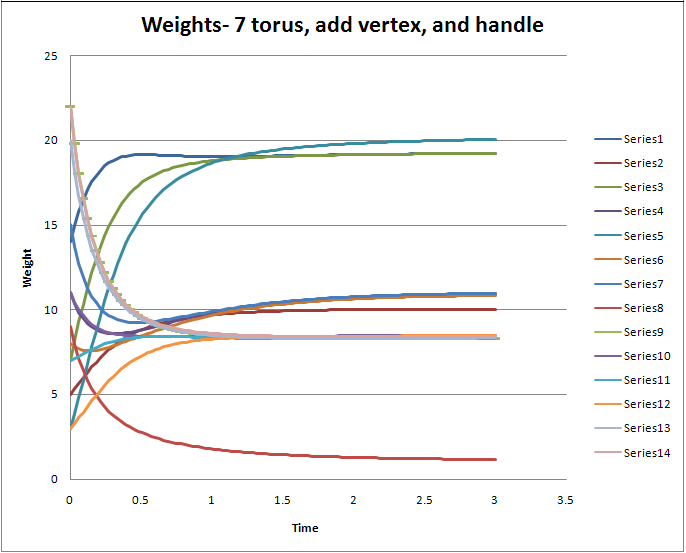
\includegraphics[scale = 0.65]{torus7addvaddhweights2.png}
\caption{An example of how morphs can change the asymptotic behavior of vertices. In this case we saw the weights of some vertices change concavity.}
\label{fig:t7vh}
\end{center}
\end{figure}

\begin{figure}
\begin{center}
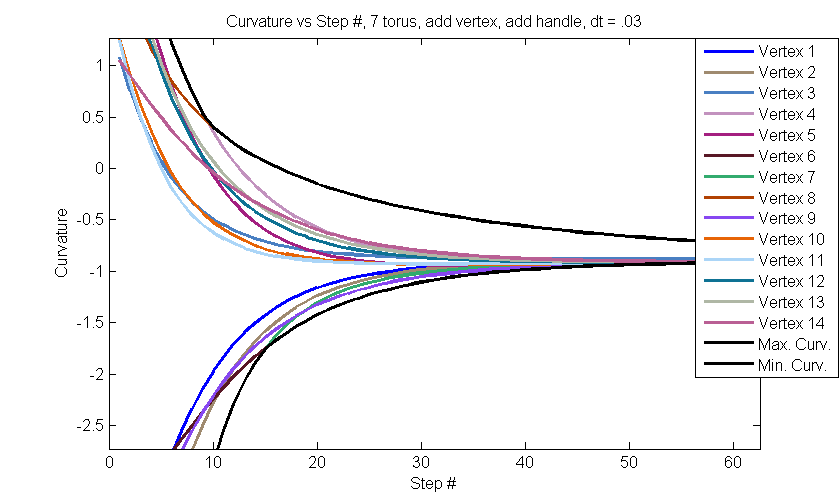
\includegraphics[scale = 0.8]{curvcurves.png}
\caption{An example of curvatures over time. While they do converge to the same curvature, the vertex with the maximum or minimum curvature may change. This is a separate trial than that producing Fig.~\ref{fig:t7vh}}
\end{center}
\end{figure}

\begin{figure}
\begin{center}
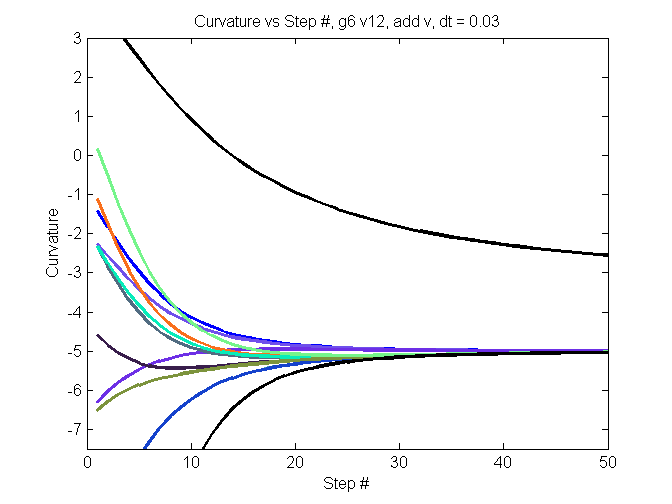
\includegraphics[scale = 0.8]{Curvg6v12addv.png}
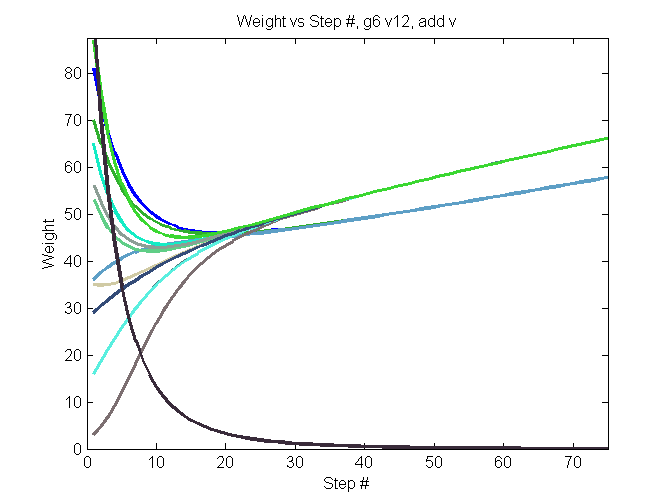
\includegraphics[scale = 0.8]{Weightg6v12addv.png}
\caption{An example of adding a vertex to a genus 6 surface. One of the curvatures in unable to drop below $-\pi$, and as a result, its weight is pushed to almost zero. Other vertices group together to compensate for this behavior.}
\end{center}
\end{figure}

%\newpage
\subsection{Code Examples}
\label{calcFlowCode}
\begin{itemize}
\item \textbf{calcFlow}
\end{itemize}
\begin{verbatim}
void calcFlow(char* fileName, double dt ,double *initWeights,
				int numSteps, bool adjF)  
{
  int p = Triangulation::vertexTable.size(); // The number of vertices.
  double ta[p],tb[p],tc[p],td[p],z[p]; // Temporary arrays to hold data in.
  int    i,k; // ints used for "for loops".
  map<int, Vertex>::iterator vit;
  map<int, Vertex>::iterator vBegin = Triangulation::vertexTable.begin();
  map<int, Vertex>::iterator vEnd = Triangulation::vertexTable.end();
  double weights[p][numSteps];
  double curvatures[p][numSteps];
  
  ofstream results(fileName, ios_base::trunc);
  results.setf(ios_base::showpoint);
  double net = 0; // Net and prev hold the current and previous
  double prev;    //  net curvatures, repsectively.
   for (k=0; k<p; k++)
     z[k]=initWeights[k]; // z[k] holds the current weights.
   for (i=1; i<numSteps+1; i++) 
   {
    prev = net; // Set prev to net.
    net = 0;    // Reset net.
    
       for (k=0, vit = vBegin; k<p && vit != vEnd; k++, vit++)  
           // Set the weights of the Triangulation.
           vit->second.setWeight(z[k]);
       if(i == 1) // If first time through, use static method.
            prev = Triangulation::netCurvature();
       for (k=0, vit = vBegin; k<p && vit != vEnd; k++, vit++)  
       // First "for loop" in whole step calculates
       {                // everything manually, prints to file.
           weights[k][i - 1] = z[k];
           double curv = curvature(vit->second);
           curvatures[k][i - 1] = curv;
           net += curv;
           if(adjF) ta[k]= dt * ((-1) * curv 
                           * vit->second.getWeight() +
                           prev /  p
                           * vit->second.getWeight());
           else     ta[k] = dt * (-1) * curv 
                           * vit->second.getWeight();
       }
       for (k=0, vit = vBegin; k<p && vit != vEnd; k++, vit++)  
       // Set the new weights.
           vit->second.setWeight(z[k]+ta[k]/2);
       for (k=0, vit = vBegin; k<p && vit != vEnd; k++, vit++)  
       {
            if(adjF) tb[k]=dt*adjDiffEQ(vit->first, net);
            else     tb[k]=dt*stdDiffEQ(vit->first);
       }
       for (k=0, vit = vBegin; k<p && vit != vEnd; k++, vit++)  
       // Set the new weights.
           vit->second.setWeight(z[k]+tb[k]/2);
       for (k=0, vit = vBegin; k<p && vit != vEnd; k++, vit++)  
       {
            if(adjF) tc[k]=dt*adjDiffEQ(vit->first, net);
            else     tc[k]=dt*stdDiffEQ(vit->first);
       }
       for (k=0, vit = vBegin; k<p && vit != vEnd; k++, vit++)  
       // Set the new weights.
           vit->second.setWeight(z[k]+tc[k]);
       for (k=0, vit = vBegin; k<p && vit != vEnd; k++, vit++)  
       {
            if(adjF) td[k]=dt*adjDiffEQ(vit->first, net);
            else     td[k]=dt*stdDiffEQ(vit->first);
       }
       for (k=0; k<p; k++) // Adjust z[k] according to algorithm.
         z[k]=z[k]+(ta[k]+2*tb[k]+2*tc[k]+td[k])/6;
   }
   for(k=0, vit = vBegin; k<p && vit != vEnd; k++, vit++) 
   {  //Print results
      results << setprecision(6); 
      results << left << "Vertex: " << left << setw(4)<< vit->first;
      results << right << setw(3) << "Weight";
      results << right << setw(10) << "Curv";
      results << "\n------------------------------\n";
      for(int j = 0; j < numSteps; j++)
      {
              results << left <<  "Step " << setw(7) << (j + 1);
              results << left << setw(12) << weights[k][j];
              results << left << setw(12) << curvatures[k][j] << "\n";
      }
      results << "\n";
   }
   results.close();
}
\end{verbatim}
\begin{itemize}
\item \textbf{2-2 Flip}
\end{itemize}
\begin{verbatim}
void flip(Edge e)
{
     //start out by naming every object that is local to the flip
     Face f1 = Triangulation::faceTable[(*(e.getLocalFaces()))[0]];
     Face f2 = Triangulation::faceTable[(*(e.getLocalFaces()))[1]];
     
     vector<int> sameAs;
     vector<int> diff;
     
     Vertex va1 = Triangulation::vertexTable[(*(e.getLocalVertices()))[0]];
     Vertex va2 = Triangulation::vertexTable[(*(e.getLocalVertices()))[1]];
          
     diff = listDifference(f1.getLocalVertices(), f2.getLocalVertices());
     if(diff.size() == 0)
     throw string("Invalid move, operation canceled");
     Vertex vb1 = Triangulation::vertexTable[diff[0]];
     diff = listDifference(f2.getLocalVertices(), f1.getLocalVertices());
     Vertex vb2 = Triangulation::vertexTable[diff[0]];
     
     sameAs = listIntersection(va1.getLocalEdges(), vb1.getLocalEdges());
     Edge ea1 = Triangulation::edgeTable[sameAs[0]];
     sameAs = listIntersection(va2.getLocalEdges(), vb1.getLocalEdges());
     Edge eb1 = Triangulation::edgeTable[sameAs[0]];
     sameAs = listIntersection(va1.getLocalEdges(), vb2.getLocalEdges());
     Edge ea2 = Triangulation::edgeTable[sameAs[0]];
     sameAs = listIntersection(va2.getLocalEdges(), vb2.getLocalEdges());
     Edge eb2 = Triangulation::edgeTable[sameAs[0]];
     
     sameAs = listIntersection(f1.getLocalFaces(), ea1.getLocalFaces());
     Face fa1 = Triangulation::faceTable[sameAs[0]];
     sameAs = listIntersection(f1.getLocalFaces(), eb1.getLocalFaces());
     Face fb1 = Triangulation::faceTable[sameAs[0]];
     sameAs = listIntersection(f2.getLocalFaces(), ea2.getLocalFaces());
     Face fa2 = Triangulation::faceTable[sameAs[0]];
     sameAs = listIntersection(f2.getLocalFaces(), eb2.getLocalFaces());
     Face fb2 = Triangulation::faceTable[sameAs[0]];
     
     //removals
     Triangulation::vertexTable[(va1.getIndex())].removeVertex(va2.getIndex()); 
     Triangulation::vertexTable[(va2.getIndex())].removeVertex(va1.getIndex()); 
     Triangulation::vertexTable[(va1.getIndex())].removeEdge(e.getIndex()); 
     Triangulation::vertexTable[(va2.getIndex())].removeEdge(e.getIndex()); 
     Triangulation::vertexTable[(va1.getIndex())].removeFace(f2.getIndex()); 
     Triangulation::vertexTable[(va2.getIndex())].removeFace(f1.getIndex()); 
     Triangulation::edgeTable[(e.getIndex())].removeVertex(va1.getIndex()); 
     Triangulation::edgeTable[(e.getIndex())].removeVertex(va2.getIndex()); 
     for(int i = 0; i < e.getLocalEdges()->size(); i++)
     {
        Triangulation::edgeTable[(e.getIndex())]
        							.removeEdge((*(e.getLocalEdges()))[i]); 
     }
     for(int i = 0; i < va1.getLocalEdges()->size(); i ++)
     {
        Triangulation::edgeTable[(*(va1.getLocalEdges()))[i]]
        							.removeEdge(e.getIndex()); 
     }
     for(int i = 0; i < va2.getLocalEdges()->size(); i ++)
     {
        Triangulation::edgeTable[(*(va2.getLocalEdges()))[i]]
        							.removeEdge(e.getIndex());  
     }
     Triangulation::edgeTable[(eb1.getIndex())].removeFace(f1.getIndex()); 
     Triangulation::edgeTable[(ea2.getIndex())].removeFace(f2.getIndex()); 
     Triangulation::faceTable[(f1.getIndex())].removeVertex(va2.getIndex()); 
     Triangulation::faceTable[(f2.getIndex())].removeVertex(va1.getIndex()); 
     Triangulation::faceTable[(f1.getIndex())].removeEdge(eb1.getIndex()); 
     Triangulation::faceTable[(f2.getIndex())].removeEdge(ea2.getIndex()); 
     Triangulation::faceTable[(f1.getIndex())].removeFace(fb1.getIndex()); 
     Triangulation::faceTable[(fb1.getIndex())].removeFace(f1.getIndex()); 
     Triangulation::faceTable[(f2.getIndex())].removeFace(fa2.getIndex()); 
     Triangulation::faceTable[(fa2.getIndex())].removeFace(f2.getIndex()); 
     
     //additions
     Triangulation::vertexTable[(vb1.getIndex())].addVertex(vb2.getIndex()); 
     Triangulation::vertexTable[(vb2.getIndex())].addVertex(vb1.getIndex()); 
     Triangulation::vertexTable[(vb1.getIndex())].addEdge(e.getIndex()); 
     Triangulation::vertexTable[(vb2.getIndex())].addEdge(e.getIndex()); 
     Triangulation::vertexTable[(vb1.getIndex())].addFace(f2.getIndex()); 
     Triangulation::vertexTable[(vb2.getIndex())].addFace(f1.getIndex()); 
     Triangulation::edgeTable[(e.getIndex())].addVertex(vb1.getIndex()); 
     Triangulation::edgeTable[(e.getIndex())].addVertex(vb2.getIndex()); 
     for(int i = 0; i < vb1.getLocalEdges()->size(); i ++)
     {
             Triangulation::edgeTable[(e.getIndex())]
             						.addEdge((*(vb1.getLocalEdges()))[i]);
             						
             Triangulation::edgeTable[(*(vb1.getLocalEdges()))[i]]
             						.addEdge(e.getIndex()); 
     }
     for(int i = 0; i < vb2.getLocalEdges()->size(); i ++)
     {
             Triangulation::edgeTable[(e.getIndex())]
             						.addEdge((*(vb2.getLocalEdges()))[i]); 
             						
             Triangulation::edgeTable[(*(vb2.getLocalEdges()))[i]]
             						.addEdge(e.getIndex()); 
     }
     Triangulation::edgeTable[(ea2.getIndex())].addFace(f1.getIndex()); 
     Triangulation::edgeTable[(eb1.getIndex())].addFace(f2.getIndex()); 
     Triangulation::faceTable[(f1.getIndex())].addVertex(vb2.getIndex());
     Triangulation::faceTable[(f2.getIndex())].addVertex(vb1.getIndex());
     Triangulation::faceTable[(f1.getIndex())].addEdge(ea2.getIndex());
     Triangulation::faceTable[(f2.getIndex())].addEdge(eb1.getIndex());
     Triangulation::faceTable[(f1.getIndex())].addFace(fa2.getIndex());
     Triangulation::faceTable[(fa2.getIndex())].addFace(f1.getIndex());
     Triangulation::faceTable[(f2.getIndex())].addFace(fb1.getIndex());
     Triangulation::faceTable[(fb1.getIndex())].addFace(f2.getIndex());
     
}
\end{verbatim}
\section*{About the authors}

Alex Henniges is a junior double majoring in Math and Computer Science. Thomas Williams is a senior in Comprehensive Mathematics with a minor in Computer Science and a background in Math Education. Mitch Wilson is a senior majoring in Applied Math and Mechanical Engineering.

\end{document}